\documentclass[12pt]{article}

\usepackage{sbc-template}
\usepackage{graphicx,url}
\usepackage[english]{babel}
\usepackage[T1]{fontenc}
\usepackage[utf8]{inputenc}
\usepackage{amsmath,amssymb,amsfonts}
\usepackage{textcomp}
\usepackage{url}
\usepackage{verbatim}
\usepackage[table,xcdraw]{xcolor}
\usepackage[shortlabels]{enumitem}
\usepackage{fancyhdr}
\usepackage{sbgames}
\usepackage{booktabs}
\usepackage{tikz}
\usetikzlibrary{positioning,arrows.meta,shapes.geometric,calc,shadows}

% C4 Model colors and styles
\definecolor{c4person}{RGB}{8, 63, 115}
\definecolor{c4system}{RGB}{17, 119, 210}
\definecolor{c4external}{RGB}{153, 153, 153}
\definecolor{c4container}{RGB}{67, 131, 191}
\definecolor{c4database}{RGB}{67, 131, 191}

\tikzset{
    c4base/.style={
        rectangle, rounded corners=2pt, draw=white, thick,
        text=white, align=center, font=\sffamily\bfseries\footnotesize,
        drop shadow={opacity=0.2}
    },
    c4container/.style={
        c4base, fill=c4container, minimum width=2.7cm, minimum height=1.1cm
    },
    c4db/.style={
        cylinder, cylinder uses custom fill, cylinder body fill=c4database,
        cylinder end fill=c4database!80, shape border rotate=90,
        draw=white, thick, text=white, align=center,
        font=\sffamily\bfseries\footnotesize,
        minimum width=2.0cm, minimum height=1.4cm, drop shadow={opacity=0.2}
    },
    c4rel/.style={
        -{Stealth[length=2mm]}, thick, draw=gray!80, font=\sffamily\scriptsize,
        text=black!80, align=center
    }
}

\tolerance=1
\emergencystretch=\maxdimen
\hyphenpenalty=10000
\hbadness=10000

\sloppy


\trilha{Informe a Trilha} %Preencha com: Artes \& Design | Computação | Cultura | Saúde | Indústria | Educação | Tutoriais | MAGICA | WGP-Jogos
\local{Cidade/UF} % Exemplo: Manaus/AM
\ano{20XX} % Exemplo: 2024
\edicao{Edição (Romano)} %Exemplo: XXIII

\title{Evaluating Interactive LLM-Based Systems: A Reproducible Protocol for Narrative Coherence and State Consistency}

\author{[OMITTED FOR ANONYMOUS REVIEW]}

\address{[OMITTED FOR ANONYMOUS REVIEW]
  \email{[OMITTED FOR ANONYMOUS REVIEW]}
}

\begin{document}

\maketitle

\thispagestyle{plain}

\begin{abstract}
Evaluating interactive Large Language Model (LLM)-based systems, such as Game Masters in role-playing games, requires assessing multi-turn, stateful, and subjective behavior that single-turn benchmarks miss. We present a reproducible evaluation protocol based on LLM-as-a-judge over structured gameplay logs, organized around six functional requirements and a metric-driven pipeline capturing narrative quality, action-to-narration coherence, and state consistency. Experiments over 10 sessions with 3 human players and four open-weight models discriminate models by profile and identify state consistency as the primary bottleneck, demonstrating the protocol's ability to capture long-term interaction failures, with five recurring failure modes more frequent below 7B parameters.
\end{abstract}

\keywords{Large Language Models, Game AI, Evaluation, Interactive Systems, LLM-as-a-Judge.}

% =============================================================================
\section{Introduction}

Tabletop Role-Playing Games (RPGs) rely on a human Game Master (GM) to lead the narrative, arbitrate rules, and maintain world consistency. With Large Language Models (LLMs), it has become possible to partially automate these functions, creating artificial GMs capable of generating interactive narratives. However, the \textit{evaluation} of such systems remains an open challenge: narrative quality, the coherence between player actions and descriptions, and state consistency across multi-turn interactions resist objective measurement, while human evaluation suffers from scalability, cost, and reproducibility limitations.

To automate this task, recent studies use LLMs as evaluators (\textit{LLM-as-a-judge}). RPGBench \cite{yu:2025} introduces RPG-specific metrics, but its evaluation is applied to controlled, single-turn scenarios rather than full interactive sessions involving multiple turns, stateful memory, and a player-driven storyline.

This work proposes an automatic evaluation pipeline applied to real RPG sessions over structured logs, with metrics adapted from RPGBench. The contribution is a \textbf{reproducible evaluation protocol for LLM-based Game Masters in interactive RPGs}, materialized in the \texttt{rpg\_judge.py} module, executing entirely on local models to eliminate dependence on cloud services, and covering combat, dialogue, and open-world exploration. The protocol is organized around six explicit functional requirements and a weighted metric system whose defaults are derived from RPGBench but redistributed for the multi-turn context.

% =============================================================================
\section{Related Works}
\label{sec:related}

\textbf{LLMs in Games.}
Gallotta et al. \cite{gallotta:2024} survey LLMs in games (content generation, NPCs, interactive narratives). Recent Brazilian work explores LLMs in narrative games \cite{sbgames:llm:2025} and RAG for tabletop dialogue \cite{sbgames:tabletop:2025}. Pre-LLM NPC behavior was typically modeled with Behavior Trees \cite{agis:2020}.

\textbf{LLMs as RPG Game Masters and Evaluation.}
Acharya et al. \cite{acharya:2023} target assistance to human GMs; we instead investigate autonomous replacement with subsequent automatic evaluation. Yu et al. \cite{yu:2025} propose RPGBench, the benchmark whose metrics for narrative quality, state consistency, and action coherence we adapt and extend to multi-turn sessions.

\textbf{LLM-as-a-Judge.}
Zheng et al. \cite{zheng:2023} validate LLMs as evaluators in MT-Bench (correlation $>80\%$ with human judgment). Reviriego et al. \cite{reviriego:2024} show that lexical diversity metrics (TTR, MTLD) complement semantic evaluation.

\textbf{Interactive and Multi-turn Evaluation.}
Guan et al. \cite{guan:2025} survey evaluation of LLM agents in multi-turn conversations. Rontogiannis et al. \cite{rontogiannis:2025} propose interactive evaluation in software engineering. Xia et al. \cite{xia:2024} formalize a process model and reference architecture for continuous evaluation of LLM agents. The present work differs by focusing on stateful narrative evaluation of full RPG sessions over structured logs with 100\% local execution. Shaker et al. \cite{shaker:2016} provide the canonical reference for the procedural-generation backbone of the open-world scenario.

% =============================================================================
\section{Methodology}
\label{sec:method}

The protocol addresses the difficulty of evaluating interactive systems based on LLMs that operate across multiple turns and maintain an evolving state. Unlike static benchmarks, the central unit of evaluation is the \textit{interaction session}, and the process is designed as a post-hoc analysis of structured gameplay logs rather than real-time monitoring.

\textbf{Functional requirements.} The protocol is designed to satisfy six requirements: \textbf{R1} multi-turn evaluation (assess complete sequences, not isolated responses); \textbf{R2} state awareness (capture world-state consistency between turns); \textbf{R3} reproducibility (deterministic given the same inputs and configuration); \textbf{R4} model-agnostic operation (multiple LLM backends without modification); \textbf{R5} metric-based assessment (explicit, interpretable metrics); and \textbf{R6} scalability (multiple sessions and models with minimal manual intervention).

\textbf{Workflow.} The evaluative process follows six steps: (1) \textit{session registration}, recording interactions in a structured format with player input, GM response, interaction type, and metadata; (2) \textit{log validation}, separating events by session ID to avoid cross-session contamination; (3) \textit{event parsing}, distinguishing narrations, actions, responses, and state-dependent sequences; (4) \textit{segment selection}, picking evidence for each metric (action-response pairs for coherence, multi-turn sequences for consistency); (5) \textit{LLM-as-a-judge} application, with metric-isolated prompts and a 1--5 Likert scale plus textual justification; and (6) \textit{aggregation}, combining per-metric scores into a weighted global score.

% =============================================================================
\section{A Metric-Driven Evaluation Framework}
\label{sec:proposal}

The protocol centers on three dominant metrics that reflect the GM's primary responsibilities and three calibration metrics that monitor the evaluation pipeline itself. The weights and roles are summarized in Table~\ref{tab:metrics}.

\begin{table}[ht]
\centering
\caption{Dominant metrics of the protocol (adapted from RPGBench). Calibration metrics GS4/GS5/QC1 share the remaining 9\%.}
\label{tab:metrics}
\small
\begin{tabular}{clcc}
\toprule
\textbf{Code} & \textbf{Metric} & \textbf{Weight} & \textbf{What it assesses} \\
\midrule
GS1 & Narrative Quality            & 36\% & Richness, vocabulary, immersion \\
GS3 & Action-to-Narration Coherence & 25\% & Did the GM narrate the correct action? \\
GS6 & State Consistency             & 30\% & No contradictions across turns \\
\bottomrule
\end{tabular}
\end{table}

\textbf{Weight rationale.} The 91\% / 9\% split between dominant and calibration metrics keeps the global score focused on the GM's behavior rather than on the evaluation pipeline. Within the dominant triplet, GS1 leads because the narrative is the GM's primary deliverable, and GS6 ranks above GS3 because state consistency is empirically the most discriminative dimension across model sizes. The defaults were inspired by the RPGBench prioritization \cite{yu:2025} and redistributed for the multi-turn context, so that dimensions emerging only across a session (most notably GS6) receive a larger share than they would in a single-turn benchmark. Weights are configurable for domain-specific priorities or when scenario-specific metrics (e.g., open-world MW1/MW2) are active.

\textbf{Outputs.} The protocol produces three artifacts: per-metric Likert scores, an aggregated weighted global score, and qualitative evaluation traces (textual justifications). These support quantitative comparison across models and qualitative diagnosis of recurring failure modes.

\textbf{Architecture.} Figure~\ref{fig:architecture} shows the system architecture as a C4-style container view~\cite{brown:2024}: four Python modules form the pipeline (Registrar, Parser \& Segmenter, Judging Coordinator, Aggregator), and three persistence stores hold session logs, configuration, and final results. The decoupling allows individual stages to be inspected, cached, or re-executed.

\begin{figure}[ht]
\centering
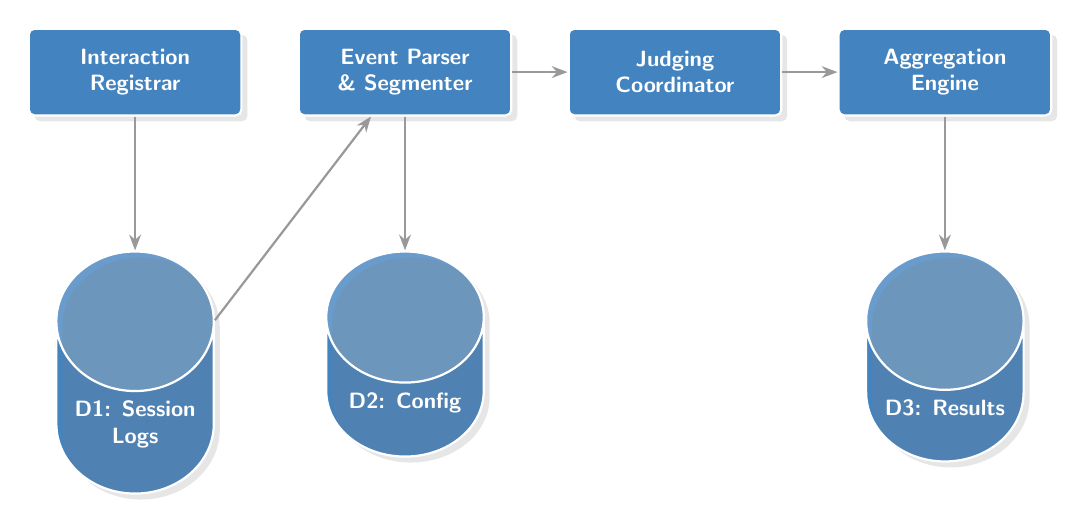
\begin{tikzpicture}[node distance=0.7cm and 0.7cm]
    % Internal Containers
    \node[c4container] (registrar) {Interaction \\ Registrar};
    \node[c4container, right=of registrar] (parser) {Event Parser \\ \& Segmenter};
    \node[c4container, right=of parser] (judgecoor) {Judging \\ Coordinator};
    \node[c4container, right=of judgecoor] (aggregator) {Aggregation \\ Engine};
    % Databases
    \node[c4db, below=1.7cm of registrar] (d1) {D1: Session \\ Logs};
    \node[c4db, below=1.7cm of parser] (d2) {D2: Config};
    \node[c4db, below=1.7cm of aggregator] (d3) {D3: Results};
    % Flows
    \draw[c4rel] (registrar) -- (d1);
    \draw[c4rel] (d1) -- (parser);
    \draw[c4rel] (parser) -- (d2);
    \draw[c4rel] (parser) -- (judgecoor);
    \draw[c4rel] (judgecoor) -- (aggregator);
    \draw[c4rel] (aggregator) -- (d3);
\end{tikzpicture}
\caption{System architecture (C4 Level~2). Four Python modules form the evaluation pipeline; three persistence stores hold session logs (CSV/SQLite), configuration (JSON), and final results (CSV/JSON).}
\label{fig:architecture}
\end{figure}

This architecture implements the evaluation pipeline used in the experiments described in Section~\ref{sec:exp}.

% =============================================================================
\section{Implementation and Experiments}
\label{sec:exp}

\textbf{Implementation.} The system is implemented in Python with \texttt{rpg\_judge.py} as the core evaluation module, accepting either a single CSV session file or a directory for batch processing, and producing two artifacts per execution: \texttt{rpg\_judge\_resultados.csv} (one record per session) and \texttt{rpg\_judge\_agregado.json} (statistics aggregated by model). Persistence uses three layers: session logs in CSV, journey state in JSON, and long-term memory in SQLite (NPC dialogue history and per-coordinate environmental facts), enabling re-injection of relevant context into the LLM rather than relying on its internal memory window. The game implementation includes three scenarios: \textit{(A)} combat with a multi-step per-turn pipeline including LLM-based creativity and efficiency assessment, streaming narration, and status effects; \textit{(B)} dialogue with NPCs, unified through \texttt{NPC.falar()} across post-battle and open-world contexts; and \textit{(C)} open-world exploration on an $(x,y,z)$ grid, with biomes determined by Euclidean distance and persistent environmental modifications by coordinate. Model integration uses a unified backend (\texttt{llm\_backend.py}) and a runtime configuration (\texttt{llm\_config.py}) supporting multiple local backends; backend and model are read at runtime per call, allowing swapping without restarts (R4). Reproducibility (R3) is supported by versioned prompts, deterministic configuration (temperature, seed, top-p), and explicit logging of model parameters per call.

\textbf{Experimental setup.} Evaluation was conducted over 10 sessions with 3 human players (30--60 rounds each), comparing four open-weight models. Table~\ref{tab:results} reports the average dominant-metric scores and the aggregated global score. Following RPGBench, scores $\geq 3.0$ mark the threshold for GM utility.

\begin{table}[ht]
\centering
\caption{Experimental results per model (Likert 1--5). $n$ = sessions evaluated; \textbf{bold} = best per column.}
\label{tab:results}
\small
\begin{tabular}{lccccc}
\toprule
\textbf{Model} & $n$ & \textbf{GS1} & \textbf{GS3} & \textbf{GS6} & \textbf{Global} \\
\midrule
\texttt{qwen2.5:7b-instruct}                           & 1 & \textbf{4.79} & \textbf{5.00} & 2.94          & \textbf{3.87} \\
\texttt{gemma4:e2b}~$^{\dagger}$ \cite{deepmind:gemma4:2026} & 1 & 4.54          & 4.84          & \textbf{2.97} & 3.70          \\
\texttt{qwen2.5:1.5b}                                  & 7 & 3.21          & 4.88          & 2.21          & 3.14          \\
\texttt{qwen2.5:0.5b}                                  & 1 & 3.34          & 3.52          & 2.04          & 3.07          \\
\bottomrule
\end{tabular}
\\[2pt]
{\footnotesize $^{\dagger}$ After adapting the parser to reasoning models (stripping \texttt{<think>} blocks and locating the last balanced JSON), reaching 100\% parse success (196/196). Before adaptation, the same model recorded Global $\approx 1.9$ due to extraction failures: integration engineering, not model capacity.}
\end{table}

\textbf{Quantitative analysis.} Table~\ref{tab:results} summarizes the evaluation results across models. Only \texttt{qwen2.5:7b-instruct} and \texttt{gemma4:e2b} cleared the $\geq 3.0$ threshold across all dominant metrics, with surprisingly close profiles: the 7B-instruct wins on GS1/GS3 while \texttt{gemma4:e2b} (effective 2B) wins on GS6, suggesting that architecture and training regime can compensate for parameter count in maintaining state. \textbf{GS6 remains the primary bottleneck}: even the best model lands at 2.97, on the threshold floor, confirming that long-term coherence is the hard limit of open-weight sub-10B models. GS3 saturates near 5.00 in models $\geq 1.5$B, indicating that simple action-coherence is well-handled. Despite the limited scale ($n=10$, four models, three scenarios), the metrics separated the four models with distinct profiles in a reproducible manner, demonstrating the protocol's discriminative capacity.

\textbf{Observed failure modes.} Qualitative analysis revealed five systematic patterns, more frequent in models below 7B: \textit{(i)} \textbf{internal-variable leakage} (\texttt{qwen2.5:0.5b} added an unsolicited JSON field, \texttt{"needs\_engaging\_context"}); \textit{(ii)} \textbf{history-contaminated hallucination} (an incorrect player name propagated across sessions and models); \textit{(iii)} \textbf{persona breaks with meta-apologies} (\texttt{qwen2.5:1.5b} replied as a technical assistant: \textit{``I apologize for the previous confusion...''}); \textit{(iv)} \textbf{log-prefix leakage} (\texttt{gemma4:e2b} reproduced structural labels \texttt{Yara:}, \texttt{Fe:}); and \textit{(v)} \textbf{admission of technical limitations} (\textit{``I don't have the capacity''} instead of building a narrative barrier).

\textbf{Limitations.} LLM-as-a-judge is not ground truth and is subject to evaluator bias, prompt sensitivity, and circularity, mitigated by using a different model as judge (\texttt{qwen2.5:7b-instruct}) and leaving formal human immersion scales for future validation \cite{zheng:2023}. Therefore, results should be interpreted as evidence of protocol validity rather than definitive model ranking.

% =============================================================================
\section{Conclusion}
\label{sec:conclusion}

This work presented a reproducible evaluation protocol for LLM-based Game Masters, materialized in \texttt{rpg\_judge.py} and operating over an autonomous GM system with combat, dialogue, and open-world scenarios on local LLMs. The three-layer persistence architecture (SQLite, JSON, CSV) supports narrative consistency, and the weighted metrics (GS1, GS3, GS6 dominant) discriminate models with distinct profiles in a reproducible manner. The protocol is not restricted to RPGs: its structure of structured logs, weighted metrics, and LLM-as-a-judge is directly applicable to other stateful interactive systems, including narrative assistants, long-duration conversational agents, and educational role-play simulations. As future work, we intend: human validation correlating automatic metrics with subjective immersion, multi-judge consensus to reduce circularity, lexical-diversity refinement (TTR, MTLD) \cite{reviriego:2024}, integration of FAISS vector databases for long-term semantic memory, and expansion of Scenario~C with complex dialogue encounters in the procedurally generated world.

\textbf{Acknowledgments.} [OMITTED FOR ANONYMOUS REVIEW]

\bibliographystyle{sbc}
\bibliography{Referencias/referencias}

\end{document}
